\documentclass[12pt]{article}


\usepackage{graphicx}
\graphicspath{ {./img/} }

\usepackage[margin=1.25in]{geometry}

\usepackage[english,ngerman]{babel}

% box for functions
\usepackage[dvipsnames]{xcolor}
\usepackage[most]{tcolorbox}
\usepackage{hyperref}
\newtcolorbox{mybox}[2][]{%
  attach boxed title to top left
               = {yshift=-8pt},
  colback      = blue!5!white,
  colframe     = blue!75!black,
  fonttitle    = \bfseries,
  colbacktitle = gray!85!black,
  title        = #2,#1,
  enhanced,
}


\author{\\ Burenko Anton \\ s76905 \\ \\ \\ Prof. Dr. Wolfgang Oertel \\ 
Computergrafik 1 \\ \\
}

\date{Wintersemester 2018/19}
\title{Belegarbeit\\ "Sunset Pagoda"}

\begin{document}
\selectlanguage{ngerman}

\maketitle

\pagebreak

\tableofcontents

\pagebreak

\section{Aufgabenstellung}
Schreiben Sie ein Programm in C/C++, das unter Verwendung von OpenGL, Vertex- und
Fragment-Shadern folgende Aufgaben realisiert. \\ \\
\textbf{Aufgabe 1}: \\
Geometrische Objekte: Erzeugen Sie eine interaktive zeitlich animierte Szene mit mehreren
unterschiedlichen farblichen und texturierten dreidimensionalen geometrischen Objekten. \\ \\
\textbf{Aufgabe 2}: \\
Beleuchtung: Beleuchten Sie die Szene mit mehreren Lichtquellen so, dass auf den Objekten
unterschiedliche Beleuchtungseffekte sichtbar werden. \\ \\
\textbf{Aufgabe 3}: \\
Ansicht: Stellen Sie die Szene gleichzeitig in verschiedenen Ansichten und Projektionen in
mehreren Viewports des Anzeigefensters dar. \\ \\
\textbf{Aufgabe 4}: \\
Programm: Stellen Sie das komplette Programm in Quelltextform als Visual-Studio-C++ -
Projekt und in ausführbarer Form als exe-File derart bereit, dass die Lauffähigkeit auf den
Computern des Praktikumslabors der Lehrveranstaltung gewährleistet ist. \\ \\
\textbf{Aufgabe 5}: \\
Dokumentation: Fertigen Sie eine Systemdokumentation in Form eines pdf-Dokumentes von
etwa 10 Seiten an, die Deckblatt, Gliederung, Aufgabenbeschreibung, Lösungsansatz,
Lösungsumsetzung, Installations- und Bedienungsanleitung, einige Bildschirm-Snapshots,
Probleme, Ergebnisse, Literatur- und Quellenverzeichnis enthält. \\ \\
\textbf{Aufgabe 6}: \\
Abgabe: Demonstrieren Sie die Ergebnisse der Aufgaben 4 und 5 an einem Computer des
Praktikumslabors der Lehrveranstaltung und übergeben Sie diese in einem Verzeichnis
$"Name\_Vorname\_Bibliotheksnummer"$. \\ \\
\textbf{Zeitplan}: \\
Die Ausgabe der Aufgabenstellung erfolgt zu Beginn der Lehrveranstaltungszeit. Die Abgabe
der Ergebnisse erfolgt spätestens zum Ende der Lehrveranstaltungszeit. \\

\pagebreak

\section{Function}
\begin{mybox}[colback=white]{setSocketTimeout}
\textbf{void setSocketTimeout(DatagramSocket ds, int time)} \\
sets timeout of socket ds to time. \\
after timeout socket throws SocketTimeoutException. \\
\textbf{Parameters:} \\
ds - DatagramSocket on wich timeout is need to be changed.  \\
time - time for timeout in ms.
\end{mybox}


\pagebreak
\section{Figure}
Für diese Szene sind 3 Figuren verwendet: ein Würfel, eine Piramide und einen Pyramidenstumpf. Alle Figuren haben eine neutrale Farbe, die danach mit einem Texture überdeckt wird. \\
\subsection{Würfel}
Der Würfel wird für Grass, Sonne und Gebäudeblocke verwendet.
\subsection{Piramide}
Die Piramide ist nur für Dach von Pagode verwendet.
\subsection{Pyramidenstumpf}
Der Pyramidenstumpf ist für den Zwischendach von Pagode verwendet.

\pagebreak

\section{Texture}
Es gibt folgende Texturen: roof, wall, grass and sun. \\
\textbf{roof} \newline
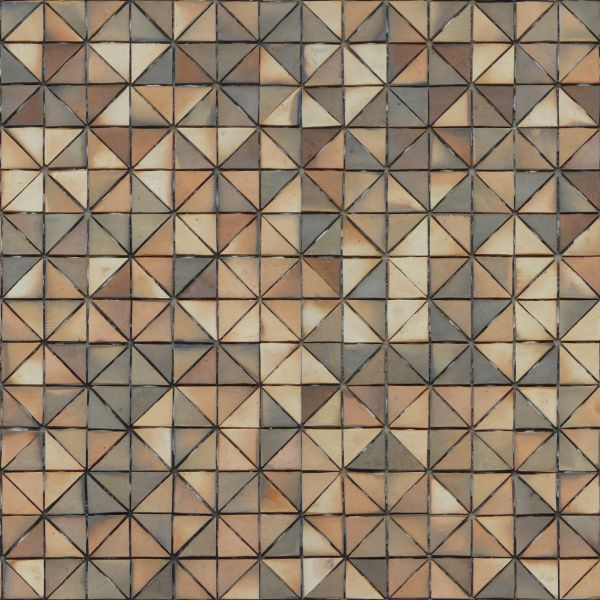
\includegraphics[width=4cm, height=4cm]{roof} \\
\textbf{wall} \newline
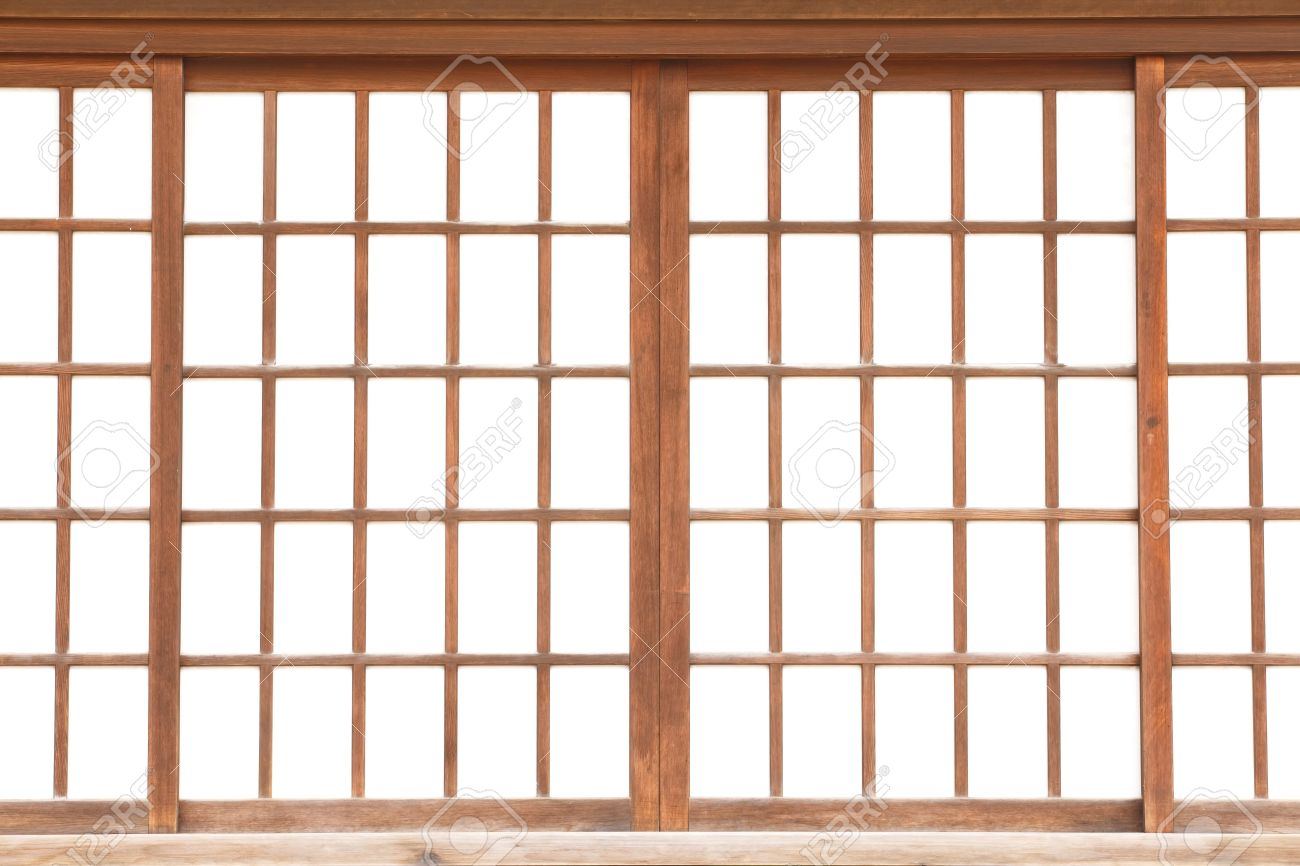
\includegraphics[width=8cm, height=4cm]{japwall} \\
\textbf{grass} \newline
\includegraphics[width=4cm, height=4cm]{grass} \\
\textbf{sun} \newline
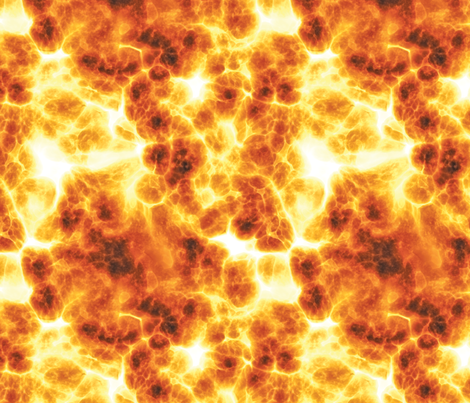
\includegraphics[width=4cm, height=4cm]{sun}

\pagebreak
\section{Light}
Die Szene enthält drei Lichtquellen: Ambiente licht, Spotlicht und Richtungslicht.
Alle Lichtquellen sind in dem Fragment Shader implementiert.
\subsection{Ambiente Licht}
\paragraph{Position} Ambiente Licht gibt es überall auf der Szene. \\\\
In dieser Szene wechselt es die Farbe von Weiß auf Rot und umgekehrt(siehe \textbf{Animation}), um den Sonnenuntergang zu simulieren.
\subsection{Spotlicht}
\paragraph{Position} Bewegt sich mit der Sonne zusammen.\\\\ 
Das Spotlicht sieht wie ein Lichtkreis von der Richtung von der Sonne aus. Die Lichtquelle bewegt sich mit dem Licht zusammen (siehe \textbf{Animation}).
Die Weiße Farbe wird vom Zenter bis Rand immer schwacher. 
\subsection{Richtungslicht}
\paragraph{Position} $(4,4,4)$ Orientiert von der Sonne rechts oben.\\\\ 
Richtungslicht kann man sehr gut als Blicke auf dem Dach beachten. Die Blicke kann man nur auf zwei Seiten sehen, weil das Licht nur aus einer Seite die Pagode beleuchtet. Am besten ist es zu sehen wenn man das Spotlicht ausmacht (siehe \textbf{Interaction}).

\pagebreak

\section{Animation}
Animation kann man schon am Anfang der Szene sehen. Die Sonne bewegt sich an der Y-Achse nach oben bzw. unten. \\
Außerdem ändert sich die Farbe dabei, um Sonnenuntergang zu simulieren.
Wenn die Sonne schon unter Niveau vom Grass-block bzw. der Erde ist wird die Farbe rot.

\pagebreak

\section{Interaction}
Die Szene kann man mit Mouse sowie mit Keyboard steuern.\\\\
\textbf{Keyboard mapping} \\\\
Z ... kleiner \\\\
V ... größer \\\\
D ... Tiefenbuffer an/aus \\\\
1 ... Richtungslich und Ambiente Licht an/aus \\\\
2 ... Spotlicht an/aus

\end{document}
\pagebreak
 